	Das dynamische Verhalten des Systems wird mittels Sequenzdiagrammen modelliert.
	Hier wird zunächst ein grobes geräteübergreifendes Diagramm vorgestellt.
	Die restlichen Sequenzdiagramme beziehen sich nur auf wichtige Methoden in den gekapselten Ökosystemen APP, Website und Backend. Deswegen werden Lost und Found Messages verwendet, um die Kommunikation mit dem Server darzustellen. 
	
\section*{Geräteübergreifendes Sequenzdiagramm}

\begin{figure}[h]
	\centering
	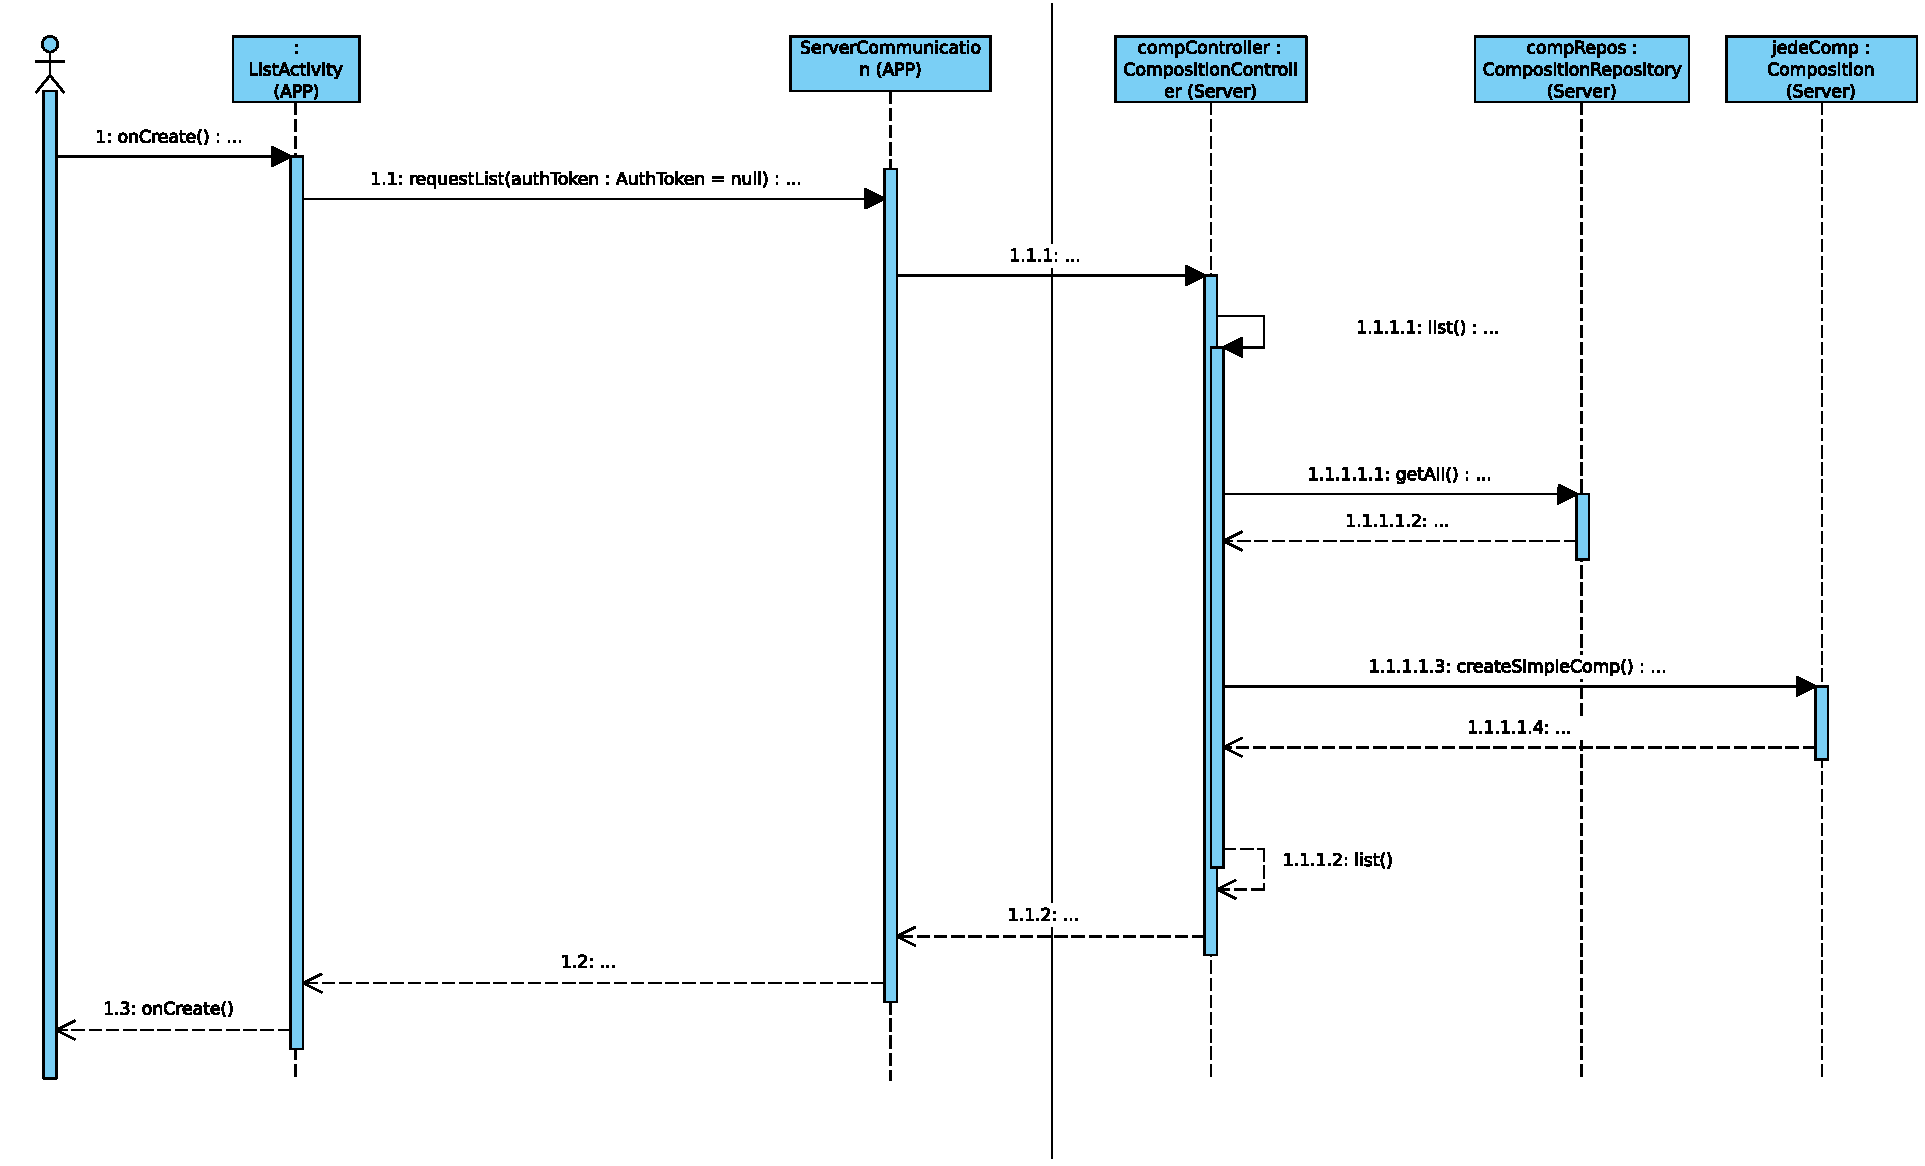
\includegraphics[width=\textwidth]{img/Diagramme/Sequenz/Overview}
	\caption{Sequenzdiagramm}
	\label{fig:sequenz-overview}
\end{figure}
\noindent
Der Benutzer öffnet die App, wodurch die Methode onCreate() der ListActivity aufgerufen wird. Zum Start wird ein HTTPS-Request an den Server gesendet. Der Server fragt die Daten aus der Datenbank ab und erstellt dazu ein versendbares Objekt in Form einer Liste von SimpleComp. Dies wird im Rahmen der Beantwortung des GET-Requests an die App geschickt. Die App verarbeitet die erhaltenen Daten, sodass sie dem Benutzer angezeigt werden können.

\section*{Sequenzdiagramme der App}
\subsection*{Sequenzdiagramm: Öffnen der ListActivity}

\begin{figure}[h]
	\centering
	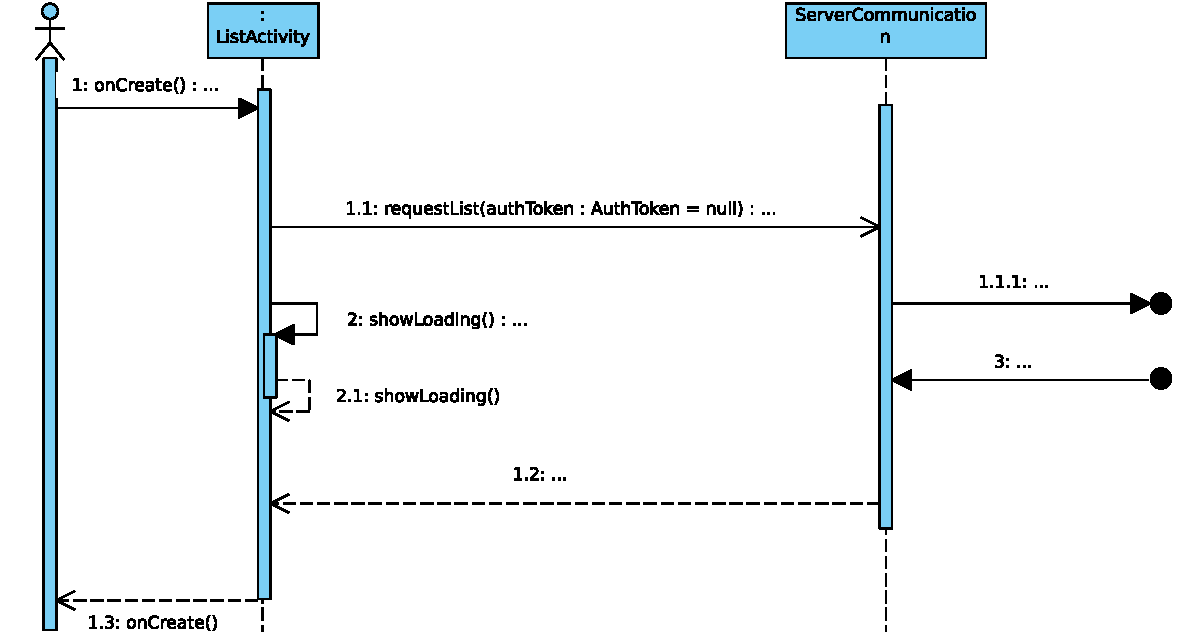
\includegraphics[width=\textwidth]{img/Diagramme/Sequenz/App_list}
	\caption{Sequenzdiagramm - Öffnen der ListActivity}
	\label{fig:sequenz-app_list}
\end{figure}
\noindent
Dieses Sequenzdiagramm zeigt den Vorgang, der abläuft, wenn die ListActivity initial gestartet wird und mit einer Liste aus Kompositionseinträgen zu füllen ist.
Da der Nutzer noch nicht eingeloggt ist, wird eine requestList()-Anfrage ohne Token gestartet. Diese wird in einem eigenen Thread ausgeführt, damit der UI-Thread nicht blockiert. Die Methode requestList() führt einen HTTPS-Request an das Backend aus. In der Zeit, in der die ListActivity die Antwort noch nicht erhalten hat, zeigt sie mithilfe von showLoading() eine Ladeanimation an.

\subsection*{Sequenzdiagramm: Klicken auf Kompositionseintrag}

\begin{figure}[h]
	\centering
	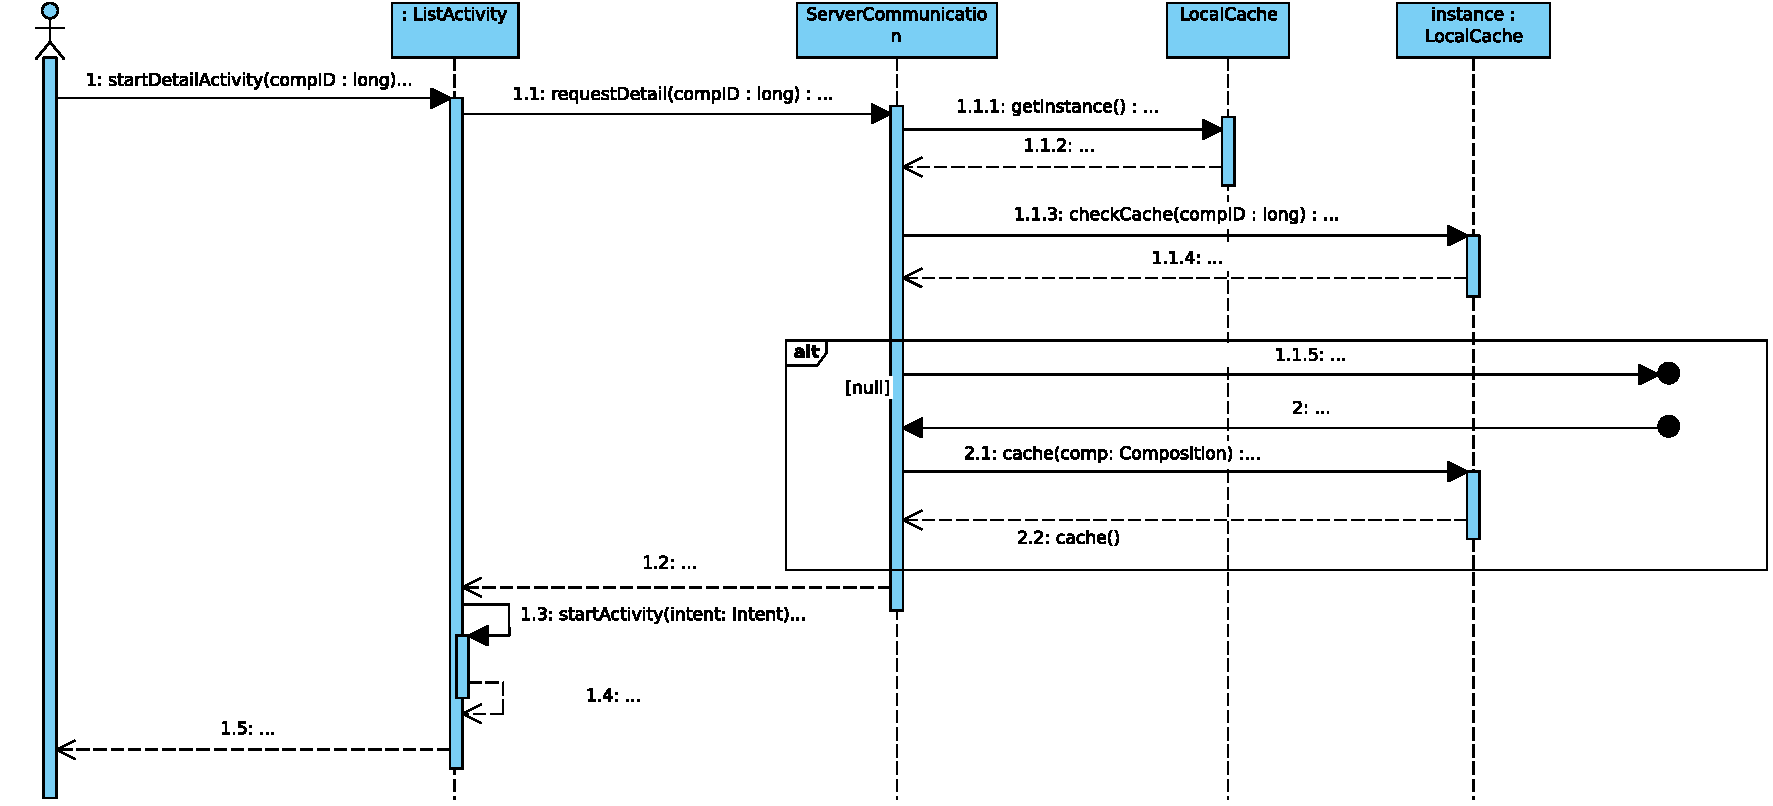
\includegraphics[width=\textwidth]{img/Diagramme/Sequenz/App_detail}
	\caption{Sequenzdiagramm - Klick auf Kompositionseintrag}
	\label{fig:sequenz-App_detail}
\end{figure}
\noindent
Dieses Sequenzdiagramm beginnt damit, dass der Nutzer auf ein Listenelement tippt, um die Detailansicht aufzurufen. 
Dadruch wird die Methode startDetailActivity() aufgerufen, die die Klasse ServerCommunication veranlasst, im LokalCache nach der gewünschten Komposition zu suchen.
Falls diese noch nicht im Cache ist, wird ein HTTPS-Request an den Server gesendet.
In der Antwort sind dann alle nötigen Details der Komposition enthalten.
Diese werden dann im LokalCache abgelegt und an die ListActivity zurückgegeben.
Damit wird dann ein Intent erstellt und die DetailActivity gestartet.
\\
Da LocalCache ein Singleton ist, muss zu Beginn die Instanz abgerufen werden. Wir planen die Instanz vorzudefinieren (eager instantiation), wodurch der Fall, dass die Instanz erst erzeugt werden muss, nie eintritt.
\\
Die Methode httpsRequest() wird nicht implementiert, sondern dient hier zur Abstraktion. In der Implementation wird diese Abfrage asynchron ablaufen und in einem anderen Thread laufen, so dass der UI-Thread nicht blockiert wird. 

\section*{Sequenzdiagramme des Models}

\begin{figure}[h]
	\centering
	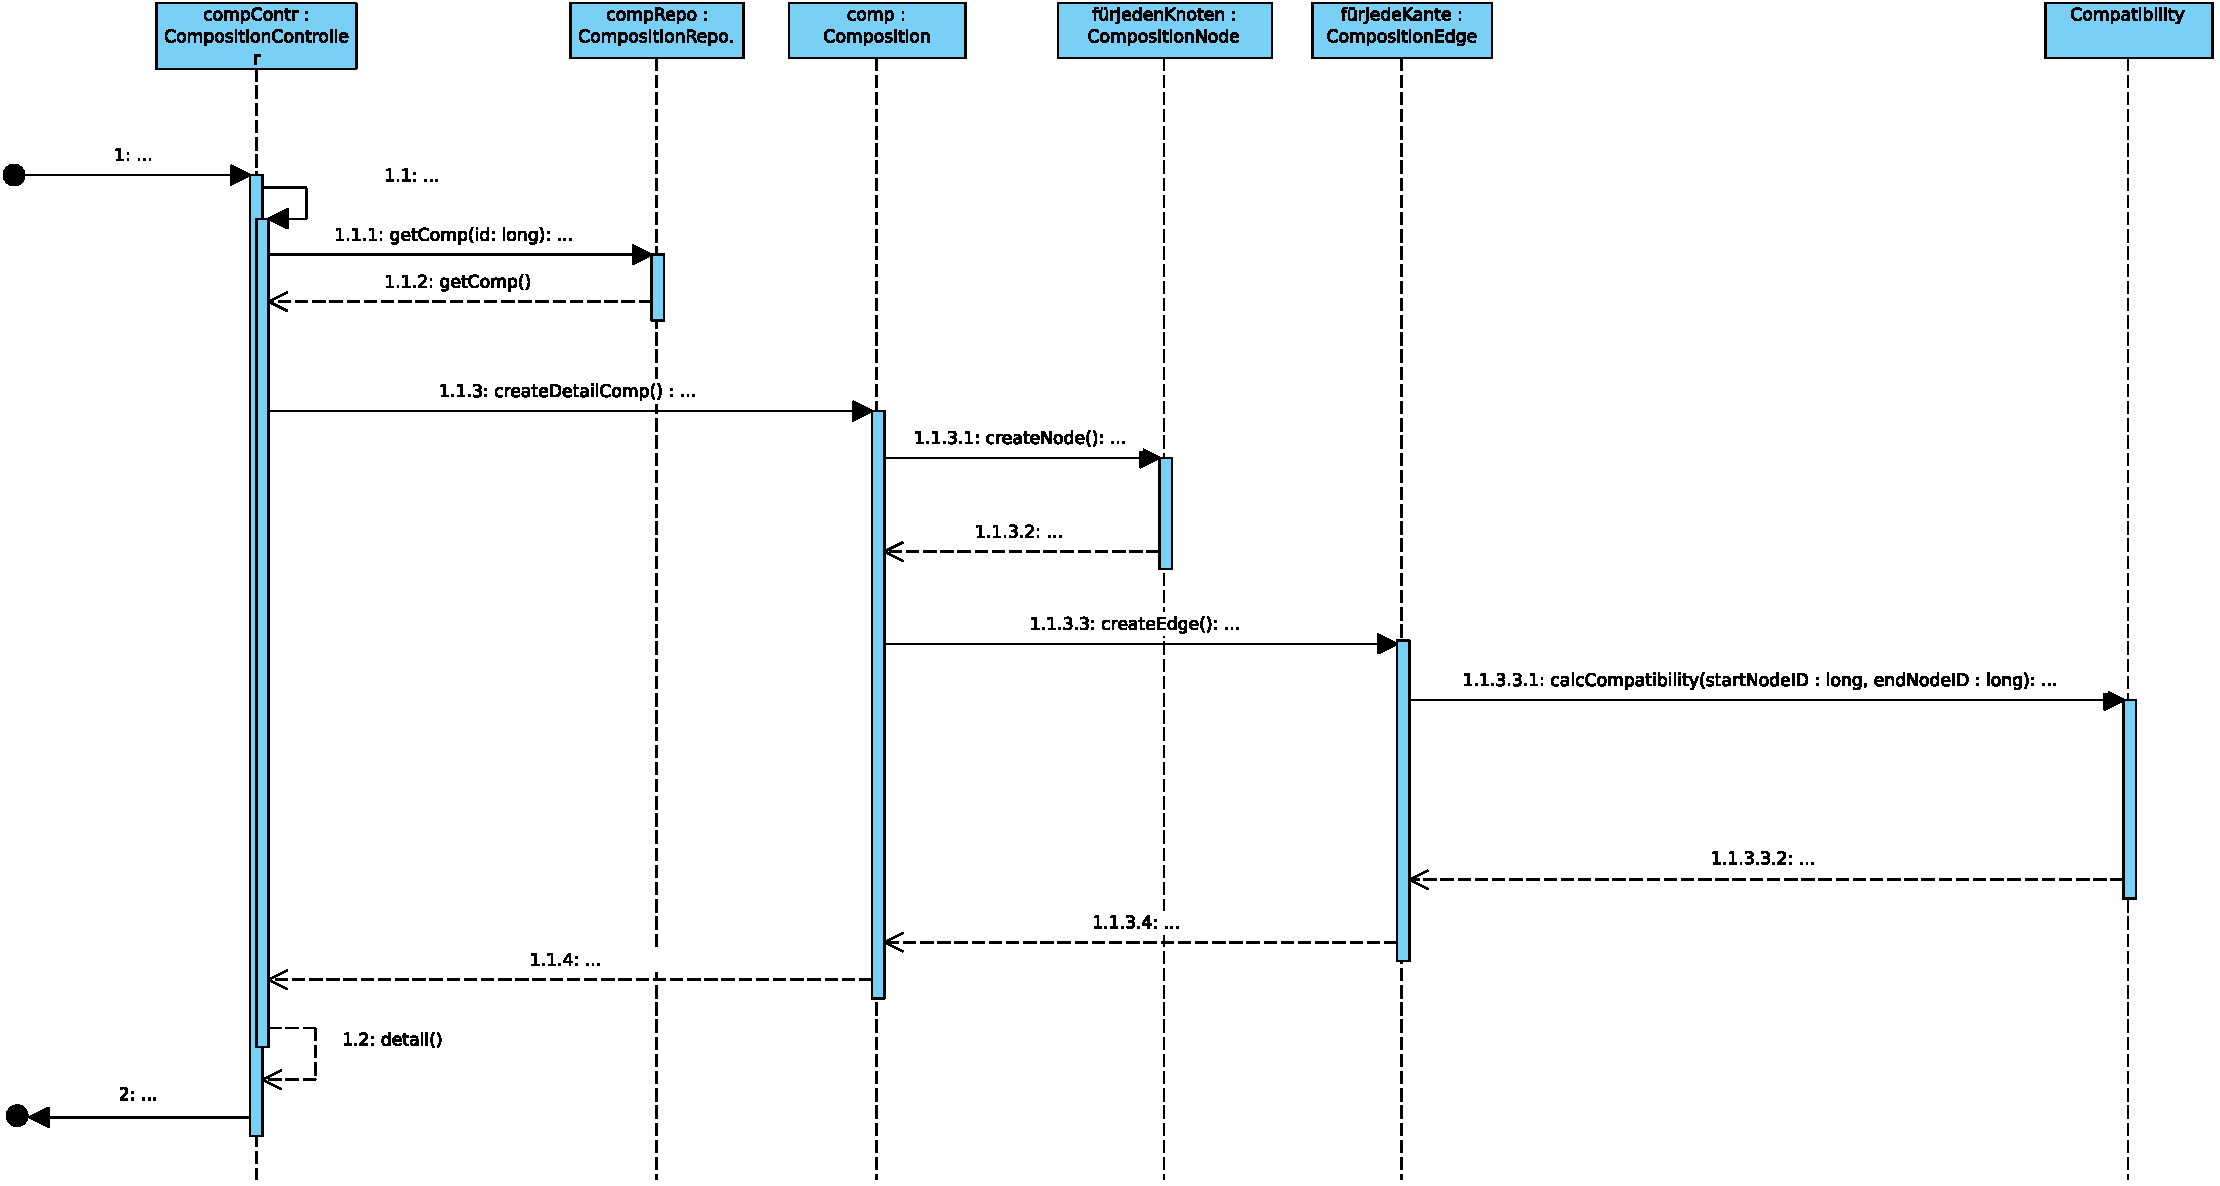
\includegraphics[width=\textwidth]{img/Diagramme/Sequenz/Controller}	
	\caption{Sequenzdiagramm - Kompositionsanfrage}
	\label{fig:sequenz-a}
\end{figure}
\noindent
Das Sequenzdiagramm zeigt, wie eine Komposition in Detailansicht angefragt wird. 
Eine solche Anfrage wird vom CompositionsController entgegengenommen.
Die angefragte Komposition wird in der Datenbank nachgeschlagen (über das CompositionRepository) und als Composition-Objekt zurückgegeben.
Anschließend wird eine DetailComp erstellt, welche die benötigten Daten für das Frontend enthält. 
Um diese zu erstellen, müssen zunächst alle CompositionNodes und danach alle CompositionEdges in versendbare Objekte (Nodes und Edges) umgewandelt werden. 
Dabei wird für jede Kante noch die Kompatibilität überprüft und mögliche Alternativen werden gesucht und ggf. gespeichert. Zurückgeliefert wird also eine DetailComp, die in allen Kanten eine CompatibilityAnswer enthält.\newline
\\ \noindent
Wir haben uns dafür entschieden, eine Util-Klasse zur Berechnung der Compatibility zwischen zwei verschiedenen Diensten (repräsentiert durch ihre IDs) zu benutzen.
Da auch HTTPS-Requests erwartet werden, die nur zu zwei einzelnen Diensten die Kompatibilität erfahren wollen, wäre eine Implementierung dieser Funktion in der Edge-Klasse unpraktisch.\newline
\\ \noindent
Da dieses Sequenzdiagramm das komplexeste ist und sich viele andere Abläufe in ihm widerspiegeln, ist hier nur dieses als Repräsentant der Arbeitsweise unseres Backends aufgeführt.

\section*{Sequenzdiagramme des Web Frontends}
\subsection*{Sequenzdiagramm: Erstellen einer Komposition}

\begin{figure}[h]
	\centering
	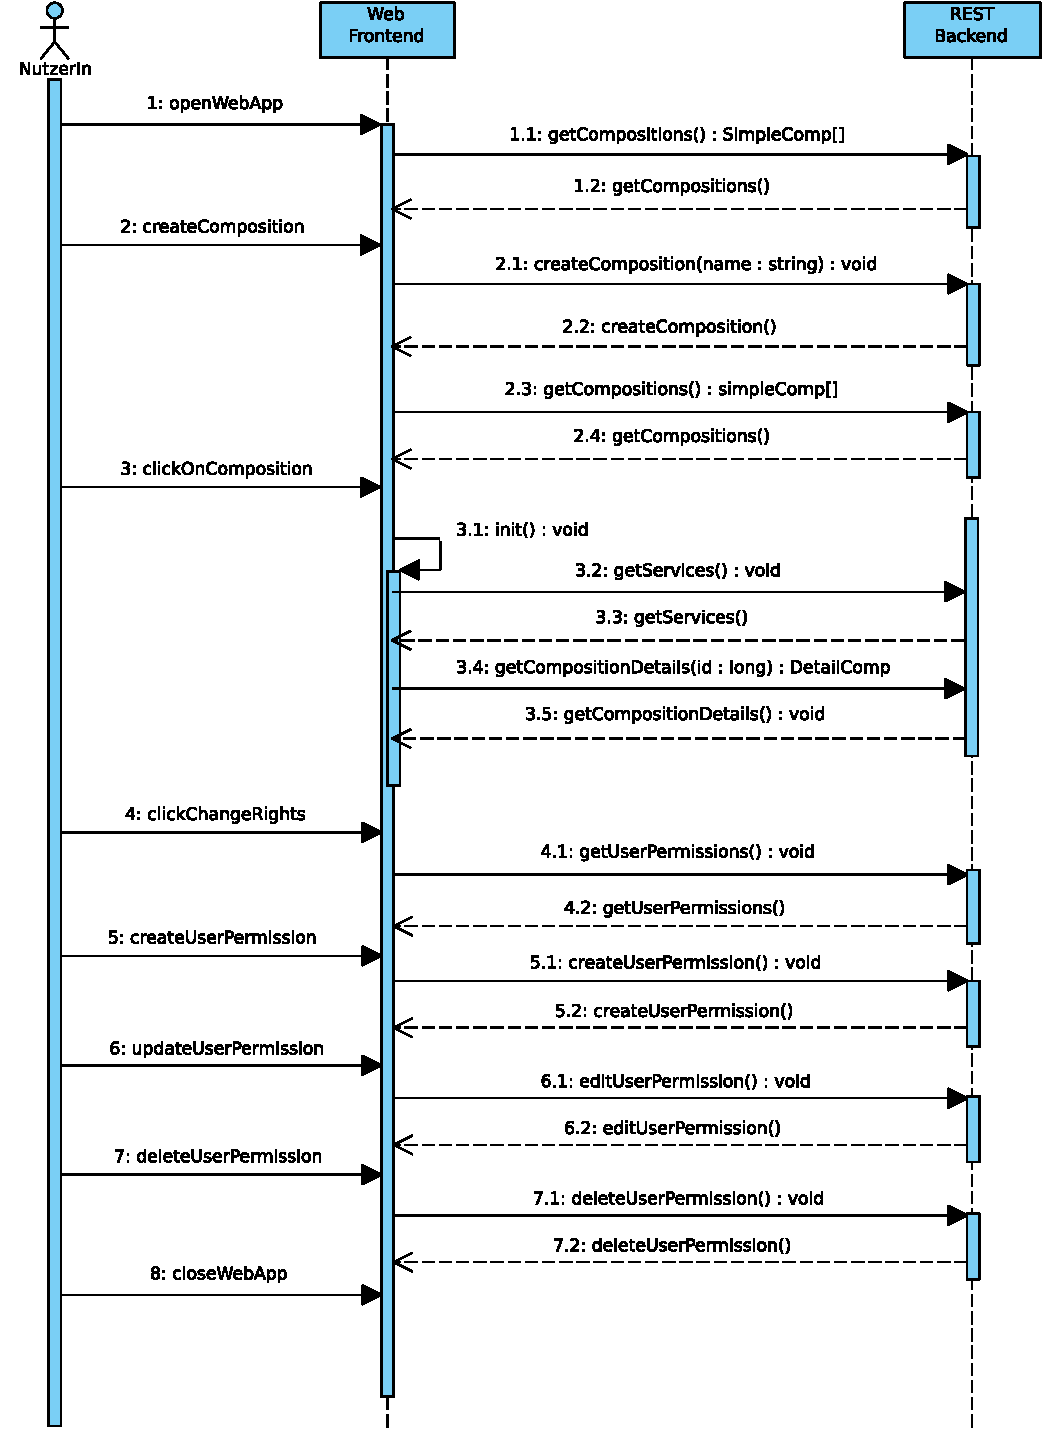
\includegraphics[width=.75\textwidth]{img/Diagramme/Sequenz/Frontend_createComp}
			
	\caption{Sequenzdiagramm - Erstellen einer Komposition}
	\label{fig:sequenz-createComp}
\end{figure}
\noindent
Um eine neue Komposition zu erstellen, werden zunächst die dem Nutzer verfügbaren Kompositionen vom Backend abgefragt und angezeigt. Über ein Eingabefeld kann ein Name für eine neue Komposition festgelegt werden und mit einem Knopf erstellt werden. Die Liste der verfügbaren Kompositionen wird refreshed und durch einen Klick auf die Komposition werden die noch leeren Details vom Backend abgerufen und in der Bearbeitungsansicht angezeigt. Als Autor der Komposition lassen sich nun die Listen mit den Nutzenden, die die Komposition einsehen oder bearbeiten dürfen, einsehen und bearbeiten. Dabei werden alle Informationen immer aus dem Backend angefordert beziehungsweise werden Aktualisierungen vom Nutzenden an das Backend geschickt.

\subsection*{Sequenzdiagramm: Bearbeiten einer Komposition}

\begin{figure}[h]
	\centering
	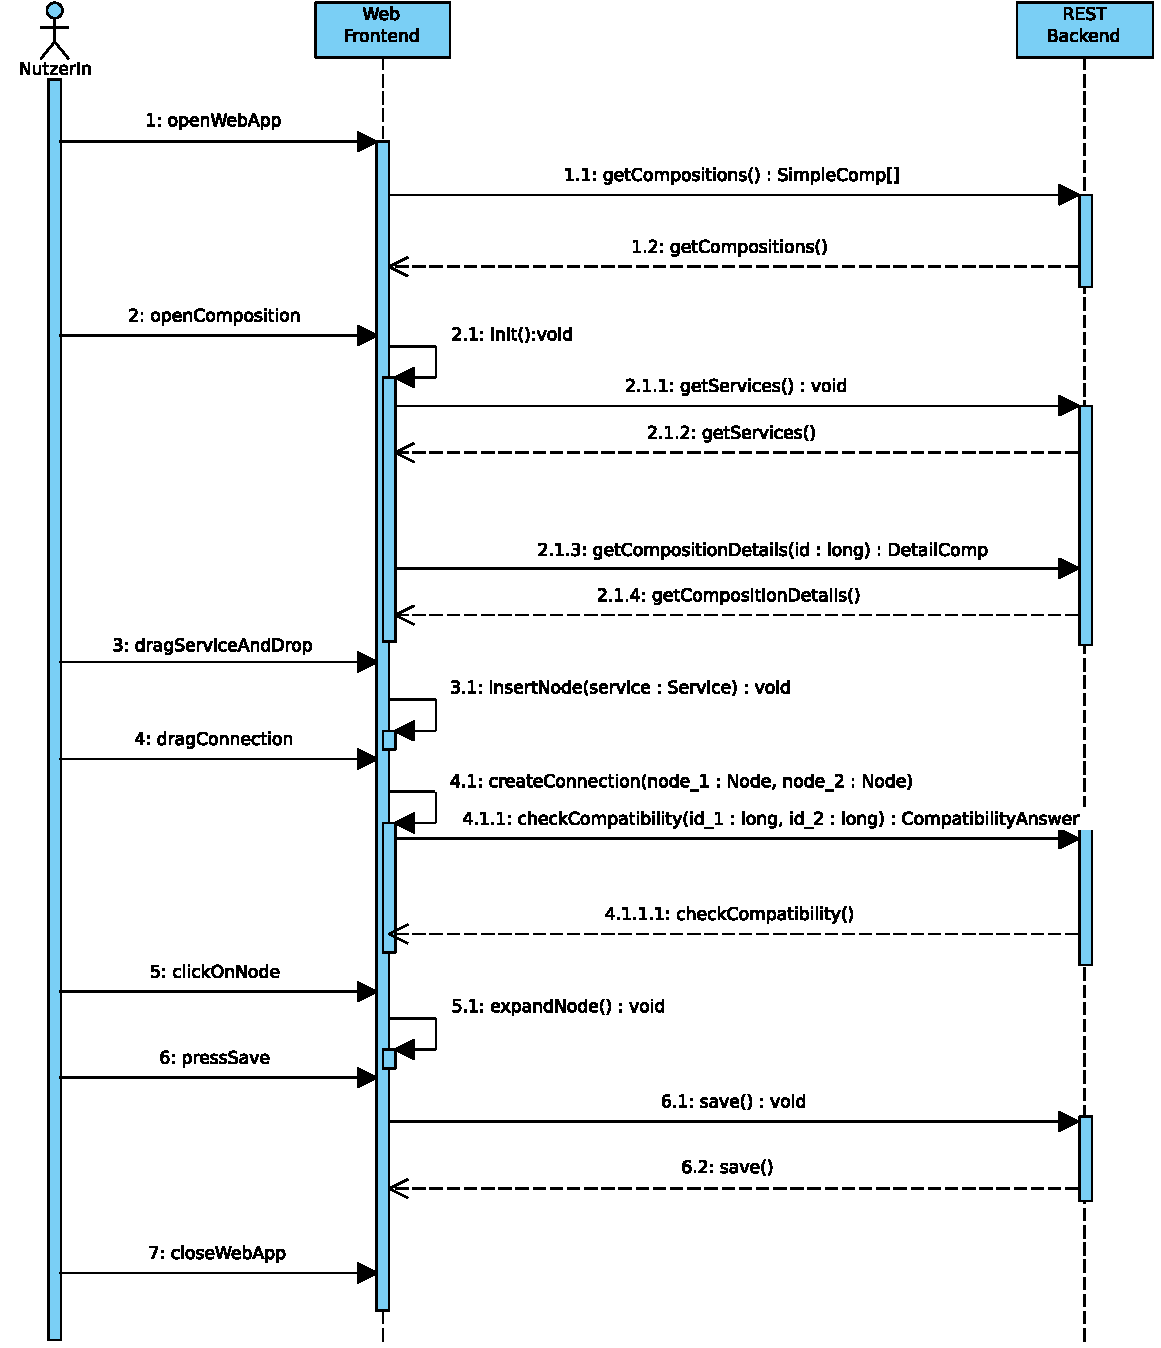
\includegraphics[width=.75\textwidth]{img/Diagramme/Sequenz/Frontend_editComp}			
	\caption{Sequenzdiagramm - Bearbeiten einer Komposition}
	\label{fig:sequenz-editComp}
\end{figure}
\noindent
Um eine Komposition zu bearbeiten, werden zunächst wieder die dem Nutzer verfügbaren Kompositionen vom Backend abgefragt und angezeigt. Durch einen Klick auf die Komposition werden die Details und Services vom Backend abgerufen und in der Bearbeitungsansicht angezeigt. Indem ein Service aus dem SidePanel in das Canvas gezogen wird, wird lokal ein Knoten erstellt. Durch das Verbinden von zwei Knoten wird zunächst lokal eine Verbindung erstellt, wobei eine Anfrage an das Backend geht, in der die Kompatibilität überprüft wird. Beim Klicken auf einen Knoten wird eine Detailansicht für den verwendeten Dienst angezeigt. Ein Klick auf Speichern sendet die aktualisierte Komposition an den Server.

\subsection*{Sequenzdiagramm: Bedienung des Adminpanels}

\begin{figure}[h]
	\centering
	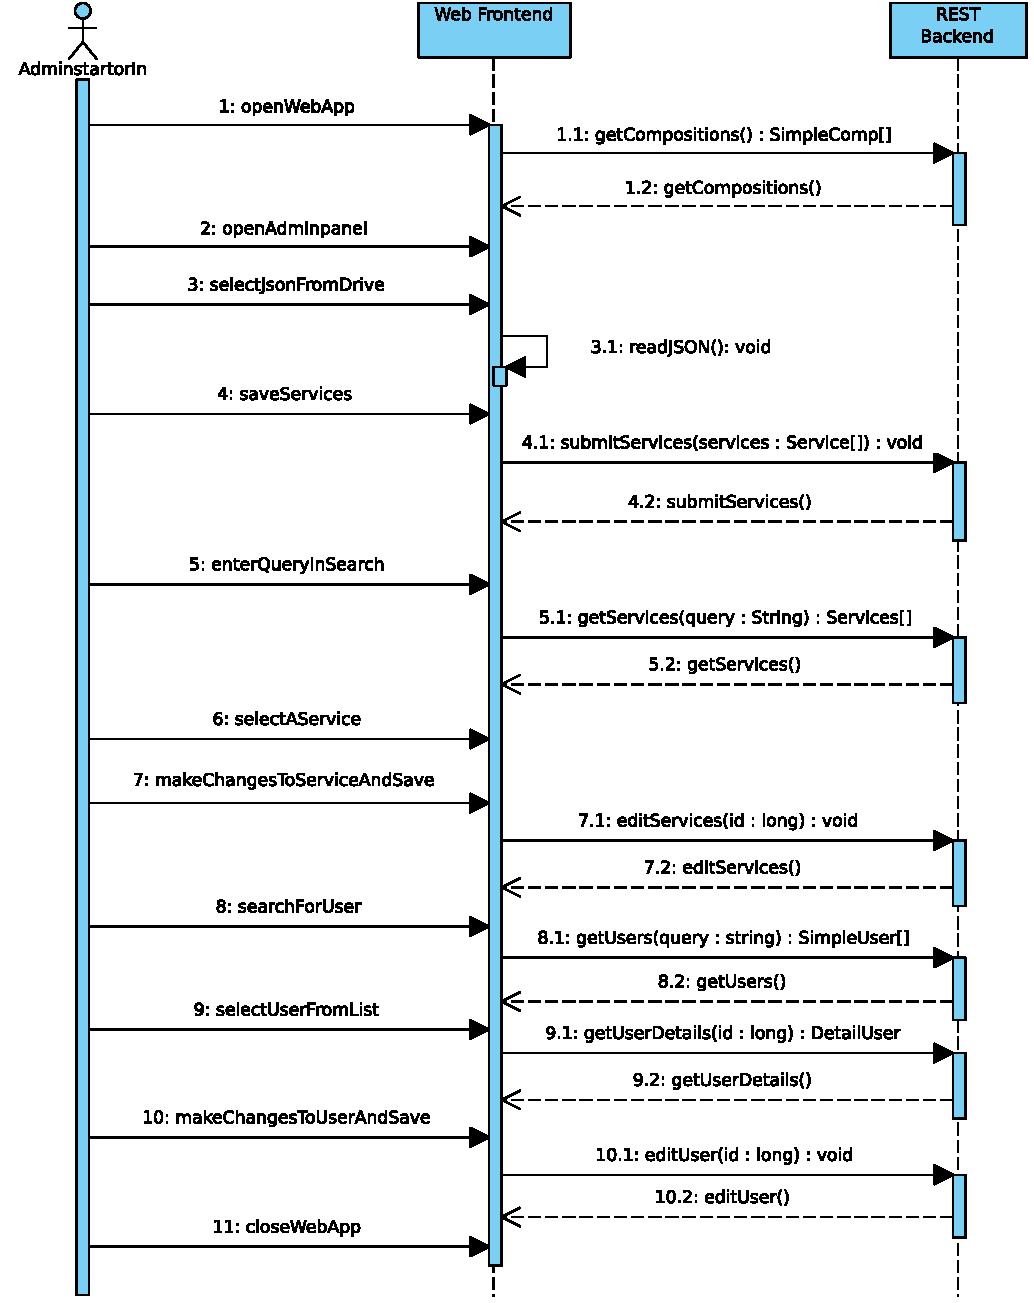
\includegraphics[width=.75\textwidth]{img/Diagramme/Sequenz/Frontend_admin}			
	\caption{Sequenzdiagramm - Bedienung des Adminpanels}
	\label{fig:sequenz-adminPanel}
\end{figure}
\noindent
Aus der Übersicht der Kompositionen wird über einen Knopf das Adminpanel erreicht. Über eine Maske lässt sich eine JSON-Datei mit Services einlesen, die zunächst nur lokal zwischengespeichert werden und dann bei Bestätigung an das Backend übermittelt werden. In einem Suchfeld für Dienste kann eine Suchanfrage an das Backend übermittelt werden, und durch Auswählen eines Listeneintrags lassen sich die Details des Services bearbeiten, die bei Bestätigung der Eingabe an das Backend gesendet werden. Weiterhin lässt sich über eine Suche nach registrierten Nutzenden suchen. Durch Auswahl eines Nutzenden werden die Details vom Backend abgefragt und lassen sich vom Adminstrierenden bearbeiten. Nach Bestätigung werden die angepassten Daten an das Backend geschickt und gespeichert.
